\documentclass[12pt]{article}

\usepackage{natbib}
\usepackage{apalike}
\usepackage[hypertexnames=false,colorlinks=true,breaklinks]{hyperref}
\usepackage{amsmath}
\usepackage{amssymb}
\usepackage{graphicx}
\usepackage[margin=1.5cm]{geometry}
\usepackage{xcolor}
\usepackage{amsthm}

\newtheorem{claim}{Claim}

\title{Inference in Linear Dynamical Systems}
\author{Joaquin Rapela\thanks{j.rapela@ucl.ac.uk}}

\begin{document}

\maketitle

\section{Linear dynamical systems (LDS) model}
\label{sec:ldsModel}

\begin{alignat*}{4}
    \mathbf{x}_n &= A \mathbf{x}_{n-1}+\mathbf{w}_n\quad && \mathbf{w}_n\sim
    N(\mathbf{w}_n|\mathbf{0}, Q)\quad && \mathbf{x}_n\in\mathbb{R}^m&&\\
    \mathbf{y}_n &= C \mathbf{x}_{n}+\mathbf{v}_n\quad && \mathbf{v}_n\sim
    N(\mathbf{v}_n|\mathbf{0}, R)\quad && \mathbf{y}_n\in\mathbb{R}^n&&\quad n=1\ldots N\\
    \mathbf{x}_0 &\sim N(\mathbf{w}_n|\mathbf{m}_0, V_0) && &&
\end{alignat*}

\begin{figure}[h]
\begin{center}
    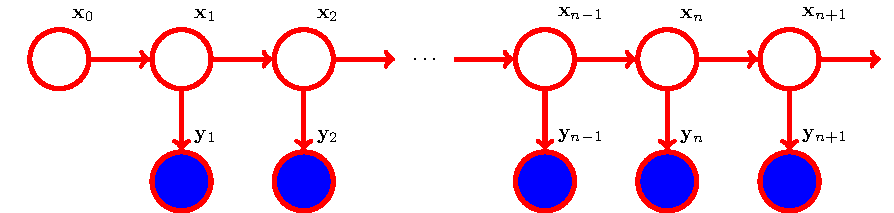
\includegraphics[width=5in]{figures/ldsGraphicalModel.pdf}
    \caption{Graphical model for linear dynamical systems}
    \label{fig:ldsGraphicalModel}
\end{center}
\end{figure}

\section{Inference Problems}
\label{sec:inferenceProblems}

\begin{description}
    \item[Prediction]
        \begin{align}
            P(\mathbf{x}_n|\mathbf{y}_1,\ldots,\mathbf{y}_{n-1})=N(\mathbf{x}_n|\mathbf{x}_{n|n-1},P_{n|n-1})\label{eq:prediction}
        \end{align}
    \item[Filtering]
        \begin{align}
            P(\mathbf{x}_n|\mathbf{y}_1,\ldots,\mathbf{y}_{n})=N(\mathbf{x}_n|\mathbf{x}_{n|n},P_{n|n})\label{eq:filtering}
        \end{align}
    \item[Smoothing]
        \begin{align}
            P(\mathbf{x}_n|\mathbf{y}_1,\ldots,\mathbf{y}_{N})=N(\mathbf{x}_n|\mathbf{x}_{n|N},P_{n|N})\label{eq:smoothing}
        \end{align}
\end{description}

\section{Kalman Filter}

The Kalman filter algorithm addresses the prediction (Eq.~\ref{eq:prediction})
and filtering (Eq.~\ref{eq:filtering}) inference problems.
%
It is an iterative algorithm, which alternates between computing the mean and
covariance of the prediction distribution and computing the mean and covariance
of the filtering distribution.

\begin{alignat*}{2}
    \mathbf{x}_{0|0}&=\mathbf{m}_0&&\text{init filtered mean}\\
    P_{0|0}&=V_0&&\text{init filtered covariance}\\
    \mathbf{x}_{n+1|n}&=A\mathbf{x}_{n|n}\quad&&\text{prediction mean}\\
    P_{n+1|n}&=AP_{n|n}A^\intercal+Q\quad&&\text{prediction covariance}\\
    \mathbf{y}_{n|n-1}&=C\mathbf{x}_{n|n-1}\quad&&\text{predicted observation}\\
    \tilde{\mathbf{y}}_n&=\textcolor{red}{\mathbf{y}_n}-\mathbf{y}_{n|n-1}\quad&&\text{residual}\\
    S_n&=CP_{n|n-1}C^\intercal+R\quad&&\text{residual covariance}\\
    \mathbf{x}_{n|n}&=\mathbf{x}_{n|n-1}+K_n\tilde{\mathbf{y}}_n\quad&&\text{filtering mean}\\
    K_n&=P_{n|n-1}C^\intercal S_n^{-1}&&\text{Kalman gain}\\
    P_{n|n}&=(I_M-K_nC)P_{n|n-1}&&\text{filtering covariance}
\end{alignat*}

Inference of predicted and filtered means and covariances proceeds in a forward
fashion, inferring the prediction and filtering distributions from the first to
the last state, as shown in the next figure.

\begin{figure}[h]
\begin{center}
    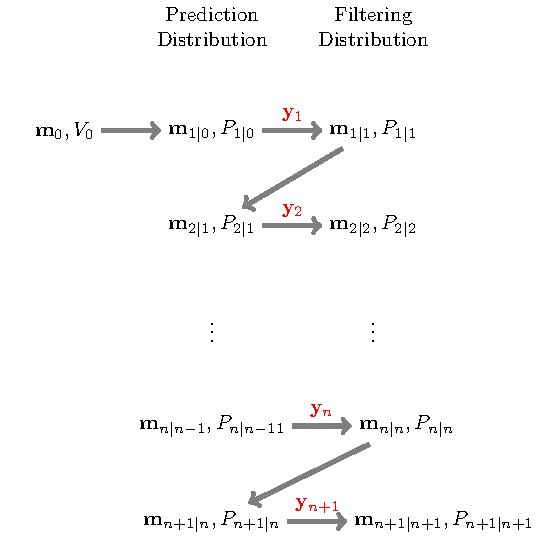
\includegraphics[width=5in]{figures/kfAlternations.pdf}
    \caption{Order of caculation of the prediction and filtering distributions
    in the Kalman filtering algorithm.}
    \label{fig:kfAlternations.}
\end{center}
\end{figure}

\section{Kalman Smoother}

The Kalman smoother algorithm addresses the smoothing (Eq.~\ref{eq:smoothing})
inference problem.

\begin{alignat*}{2}
    x_{n|N}&=x_{n|n}+C_n(x_{n+1|N}-x_{n+1|n})\quad&&\text{smoothed mean}\\
    P_{n|N}&=P_{n|n}+C_n(P_{n+1|N}-P_{n+1|n})C_n^\intercal\quad&&\text{smoothed covariance}\\
    C_n&=P_{n|n}A^\intercal P_{n+1|n}^{-1}&&
\end{alignat*}

Inference of smoothed mean and covariances proceeds in a backward fashion:
$x_{N|N}, P_{N|N}\rightarrow x_{N-1|N}, P_{N-1|N}\rightarrow x_{N-2|N},
P_{N-2|N}\rightarrow\ldots\rightarrow  x_{1|N}, P_{1|N}$. The initial mean and
covariances (i.e., $x_{N|N}, P_{N|N}$) are initialized from the last step of
the Kalman filter.

\section{Derivation of Kalman filter equations}

\begin{claim}
    $\mathbf{x}_{n|n-1}=A\mathbf{x}_{n-1|n-1}$
    \label{claim:predictionMean}
\end{claim}

\begin{proof}
    \begin{align}
        \mathbf{x}_{n|n-1}&=E\{\mathbf{x}_n|\mathbf{y}_1,\ldots,\mathbf{y}_{n-1}\}\nonumber\\
                          &=E\{A\mathbf{x}_{n-1}+\mathbf{w}_n|\mathbf{y}_1,\ldots,\mathbf{y}_{n-1}\}\label{eq:c1l2}\\
                          &=AE\{\mathbf{x}_{n-1}|\mathbf{y}_ 1,\ldots,\mathbf{y}_{n-1}\}+E\{\mathbf{w}_n|\mathbf{y}_1,\ldots,\mathbf{y}_{n-1}\}\label{eq:c1l3}\\
                          &=A\mathbf{x}_{n-1|n-1}+E\{\mathbf{w}_n\}\label{eq:c1l4}\\
                          &=A\mathbf{x}_{n-1|n-1\label{eq:c1l5}}
    \end{align}
\end{proof}

Notes:

\begin{itemize}

    \item Eq.~\ref{eq:c1l2} arises from the state equation of the LDS model in
        Section~\ref{sec:ldsModel},
    \item Eq.~\ref{eq:c1l3} holds because the expectation distributes over sums
    \item Eq.~\ref{eq:c1l4} uses the definition of $\mathbf{x}_{n-1|n-1}$ and
        the fact that the state noise, $\mathbf{w}_n$, is independent of previous observations.
    \item Eq.~\ref{eq:c1l5} follows due to the zero mean of $\mathbf{w}_n$.
\end{itemize}

\begin{claim}
    $P_{n|n-1}=AP_{n-1|n-1}A^\intercal+Q$
    \label{claim:predictionCov}
\end{claim}

\begin{proof}
    \begin{align}
        P_{n|n-1}=&\text{Cov}\{\mathbf{x}_n|\mathbf{y}_1,\ldots,\mathbf{y}_{n-1}\}\nonumber\\
                 =&\text{Cov}\{A\mathbf{x}_{n-1}+\mathbf{w}_n|\mathbf{y}_1,\ldots,\mathbf{y}_{n-1}\}\label{eq:c2l2}\\
                 =&\text{Cov}\{A\mathbf{x}_{n-1}|\mathbf{y}_1,\ldots,\mathbf{y}_{n-1}\}+\text{Cov}\{\mathbf{w}_n|\mathbf{y}_1,\ldots,\mathbf{y}_{n-1}\}\label{eq:c2l3}\\
                 =&A\ \text{Cov}\{\mathbf{x}_{n-1}|\mathbf{y}_1,\ldots,\mathbf{y}_{n-1}\}\ A^\intercal+\text{Cov}\{\mathbf{w}_n\}\label{eq:c2l4}\\
                 =&A\ P_{n-1|n-1}\ A^\intercal+Q\label{eq:c2l5}
    \end{align}
\end{proof}
Notes:

\begin{enumerate}
    \item Eq.~\ref{eq:c2l2} used the state equation of the LDS model in
        Section~\ref{sec:ldsModel},
    \item Eq.~\ref{eq:c2l3} is true because $\mathbf{w}_n$ is indepedent from
        $\mathbf{x}_{n-1}$,
    \item Eq.~\ref{eq:c2l4} holds by the property
        $\text{Cov}\{A\mathbf{x}\}=A\ \text{Cov}\{\mathbf{x}\}' A^\intercal$ and
        because $\mathbf{w}_n$ is independent of previous observations.
    \item Eq.~\ref{eq:c2l4} applied the definitions of $P_{n-1|n-1}$ and $Q$.
\end{enumerate}

\begin{claim}
    $\mathbf{x}_{n|n}=\mathbf{x}_{n|n-1}+K_n\tilde{\mathbf{y}}_n$ and
    $P_{n|n}=(I-K_nC)P_{n|n-1}$.
    \label{claim:filteringMeanAndCov}
\end{claim}

\begin{proof}

    Define the random variables
    $\mathbf{x}=\mathbf{x}_n|\mathbf{y}_1,\ldots,\mathbf{y}_{n-1}$ and
    $\mathbf{y}=\mathbf{y}_n|\mathbf{y}_1,\ldots,\mathbf{y}_{n-1}$. Then
    $\mathbf{x}|\mathbf{y}=\mathbf{x}_n|\mathbf{y}_1,\ldots,\mathbf{y}_n$ and
    the mean and covariance that we want to find, $\mathbf{x}_{n|n}$ and
    $P_{n|n}$, are those of $\mathbf{x}|\mathbf{y}$.  Thus, we want to compute
    the mean, $\mu_{\mathbf{x}|\mathbf{y}}=\mathbf{x}_{n|n}$, and covariance,
    $\Sigma_{\mathbf{x}|\mathbf{y}}=P_{n|n}$, of $\mathbf{x}|\mathbf{y}$.

    Because $\mathbf{x}_n$ and $\mathbf{y}_n$ are jointly Gaussian, then
    $\mathbf{x}$ and $\mathbf{y}$ are also jointly Gaussian. Then, $\mu_{\mathbf{x}|\mathbf{y}}$
    and $\Sigma_{\mathbf{x}|\mathbf{y}}$ are \citep[][Chapter 2]{bishop06}

    \begin{align}
        \mu_{\mathbf{x}|\mathbf{y}}&=\mu_{\mathbf{x}} +
        \Sigma_{\mathbf{x}\mathbf{y}}\Sigma_{\mathbf{y}\mathbf{y}}^{-1}(\mathbf{y}_n-\mu_{\mathbf{y}})\label{eq:muxgy}\\
        \Sigma_{\mathbf{x}|\mathbf{y}}&=\Sigma_{\mathbf{x}\mathbf{x}}-\Sigma_{\mathbf{x}\mathbf{y}}\Sigma_{\mathbf{y}\mathbf{y}}^{-1}\Sigma_{\mathbf{y}\mathbf{x}}\label{eq:sigmaxgy}
    \end{align}

    Thus, to compute $\mu_{\mathbf{x}|\mathbf{y}}$ and $\Sigma_{\mathbf{x}|\mathbf{y}}$ we need to calculate
    $\mu_{\mathbf{x}}$, $\mu_{\mathbf{y}}$, $\Sigma_{\mathbf{x}\mathbf{x}}$, $\Sigma_{\mathbf{x}\mathbf{y}}$ and $\Sigma_{\mathbf{y}\mathbf{y}}$.

    \rule{2in}{0.4pt}

    \begin{align}
        \mu_{\mathbf{x}}=E\{\mathbf{x}\}=E\{\mathbf{x}_n|\mathbf{y}_1,\ldots\mathbf{y}_{n-1}\}=\mathbf{x}_{n|n-1}\label{eq:mux}
    \end{align}

    \rule{2in}{0.4pt}

    \begin{align}
        \mu_{\mathbf{y}}&=E\{\mathbf{y}\}=E\{\mathbf{y}_n|\mathbf{y}_1,\ldots\mathbf{y}_{n-1}\}=E\{C\mathbf{x}_n+\mathbf{v}_n|\mathbf{y}_1,\ldots\mathbf{y}_{n-1}\}=\nonumber\\
             &=CE\{\mathbf{x}_n|\mathbf{y}_1,\ldots\mathbf{y}_{n-1}\}+E\{\mathbf{v}_n|\mathbf{y}_1,\ldots\mathbf{y}_{n-1}\}=C\mathbf{x}_{n|n-1}+E\{\mathbf{v}_n\}=C\mathbf{x}_{n|n-1}=\mathbf{y}_{n|n-1}\label{eq:muy}
    \end{align}

    Notes:

    \begin{itemize}
        \item The penultimate equality in Eq.~\ref{eq:muy} uses the definition
            of $\mathbf{x}_{n|n-1}$ and the fact that $\mathbf{v}_n$ is
            independent of previous observations.

        \item The last equality in Eq.~\ref{eq:muy} holds because the mean of
            $\mathbf{v}_n$ is zero.
            Claim~\ref{claim:predictionMean}.
    \end{itemize}

    \rule{2in}{0.4pt}

    \begin{align}
        \Sigma_{\mathbf{y}\mathbf{y}}&=\text{Cov}(\mathbf{y}_n|\mathbf{y}_1,\ldots,\mathbf{y}_{n-1})\nonumber\\
                                     &=\text{Cov}(C\mathbf{x}_n+\mathbf{v}_n|\mathbf{y}_1,\ldots,\mathbf{y}_{n-1})\nonumber\\
                                     &=\text{Cov}(C\mathbf{x}_n|\mathbf{y}_1,\ldots,\mathbf{y}_{n-1})+\text{Cov}(\mathbf{v}_n|\mathbf{y}_1,\ldots,\mathbf{y}_{n-1})\nonumber\\
                                     &=C\ \text{Cov}(\mathbf{x}_n|\mathbf{y}_1,\ldots,\mathbf{y}_{n-1})\ C^\intercal+\text{Cov}(\mathbf{v}_n)\label{eq:c3Sigmayyl4}\\
                                     &=CP_{n|n-1}C^\intercal+R\label{eq:sigmayy}
    \end{align}

    \rule{2in}{0.4pt}

Notes:

\begin{itemize}

    \item As in Eq.~\ref{eq:c2l3}, Eq.~\ref{eq:c3Sigmayyl4} holds by the
        property
        $\text{Cov}\{A\mathbf{x}\}=A\ \text{Cov}\{\mathbf{x}\}\ A^\intercal$ and
        because $\mathbf{v}_n$ is independent of previous observations.

\end{itemize}

    \rule{2in}{0.4pt}

    \begin{align}
        \Sigma_{\mathbf{x}\mathbf{y}}&=\text{cCov}(\mathbf{x}_n,\mathbf{y}_n|\mathbf{y}_1,\ldots,\mathbf{y}_{n-1})\nonumber\\
                                     &=\text{cCov}(\mathbf{x}_n,C\mathbf{x}_n+\mathbf{v}_n|\mathbf{y}_1,\ldots,\mathbf{y}_{n-1})\nonumber\\
                                     &=\text{cCov}(\mathbf{x}_n,C\mathbf{x}_n|\mathbf{y}_1,\ldots,\mathbf{y}_{n-1})+\text{cCov}(\mathbf{x}_n,\mathbf{v}_n|\mathbf{y}_1,\ldots,\mathbf{y}_{n-1})\label{eq:c3Sigmaxyl3}\\
                                     &=\text{Cov}(\mathbf{x}_n|\mathbf{y}_1,\ldots,\mathbf{y}_{n-1})C^\intercal+0\label{eq:c3Sigmaxyl4}\\
                                     &=P_{n|n-1}C^\intercal\label{eq:sigmaxy}
    \end{align}

    Notes:

    \begin{itemize}
        \item the first term in Eq.~\ref{eq:c3Sigmaxyl4} arises from the first
            term of Eq.~\ref{eq:c3Sigmaxyl3} since

            \begin{align*}
                \text{cCov}(\mathbf{x}_n,C\mathbf{x}_n|\mathbf{y}_1,\ldots,\mathbf{y}_{n-1})&=E\{(\mathbf{x}_n-\mu_\mathbf{x})(C\mathbf{x}_n-C\mu_{\mathbf{x}})^\intercal|\mathbf{y}_1,\ldots,\mathbf{y}_{n-1}\}\\
                                                                                            &=E\{(\mathbf{x}_n-\mu_\mathbf{x})(\mathbf{x}_n-\mu_{\mathbf{x}})^\intercal C^\intercal|\mathbf{y}_1,\ldots,\mathbf{y}_{n-1}\}\\
                                                                                            &=E\{(\mathbf{x}_n-\mu_\mathbf{x})(\mathbf{x}_n-\mu_{\mathbf{x}})^\intercal|\mathbf{y}_1,\ldots,\mathbf{y}_{n-1}\}C^\intercal\\
                                                                                            &=\text{Cov}(\mathbf{x}_n|\mathbf{y}_1,\ldots,\mathbf{y}_{n-1})C^\intercal
            \end{align*}
        \item the second term in Eq.~\ref{eq:c3Sigmaxyl4} arises from the
            second
            term of Eq.~\ref{eq:c3Sigmaxyl3} since

            \begin{align*}
                \text{cCov}(\mathbf{x}_n,\mathbf{v}_n|\mathbf{y}_1,\ldots,\mathbf{y}_{n-1})&=E\{(\mathbf{x}_n-\mathbf{x}_{n|n-1})\mathbf{v}_n|\mathbf{y}_1,\ldots,\mathbf{y}_{n-1}\}\\
                                                                                           &=E\{(\mathbf{x}_n-\mathbf{x}_{n|n-1})|\mathbf{y}_1,\ldots,\mathbf{y}_{n-1}\}E\{\mathbf{v}_n|\mathbf{y}_1,\ldots,\mathbf{y}_{n-1}\}\\
                                                                                           &=E\{(\mathbf{x}_n-\mathbf{x}_{n|n-1})|\mathbf{y}_1,\ldots,\mathbf{y}_{n-1}\}E\{\mathbf{v}_n\}\\
                                                                                           &=E\{(\mathbf{x}_n-\mathbf{x}_{n|n-1})|\mathbf{y}_1,\ldots,\mathbf{y}_{n-1}\}0\\
                                                                                           &=0
            \end{align*}

            the second line follows from the first one because $\mathbf{v}_n$
            is independent of $\mathbf{x}_n$, and the third line follows from
            the second one because $\mathbf{v}_n$ is indepednent of previous
            observations.

    \end{itemize}
    \rule{2in}{0.4pt}

    \begin{align}
        \Sigma_{\mathbf{x}\mathbf{x}}&=\text{Cov}(\mathbf{x}_n|\mathbf{y}_1,\ldots,\mathbf{y}_{n-1})=P_{n|n-1}\label{eq:sigmaxx}
    \end{align}

    \rule{2in}{0.4pt}

    Having calculated $\mu_{\mathbf{x}}$, $\mu_{\mathbf{y}}$,
    $\Sigma_{\mathbf{x}\mathbf{x}}$, $\Sigma_{\mathbf{x}\mathbf{y}}$ and
    $\Sigma_{\mathbf{y}\mathbf{y}}$ we now use Eqs.~\ref{eq:muxgy},
    \ref{eq:sigmaxgy}, \ref{eq:mux},  \ref{eq:muy},  \ref{eq:sigmayy},
    \ref{eq:sigmaxy}, and \ref{eq:sigmaxx} to  
    obtain $\mathbf{x}_{n|n}$ and $P_{n|n}$.

    \begin{align*}
        \mathbf{x}_{n|n}=\mu_{\mathbf{x}|\mathbf{y}}&=\mu_{\mathbf{x}} + \Sigma_{\mathbf{x}\mathbf{y}}\Sigma_{\mathbf{y}\mathbf{y}}^{-1}(\mathbf{y}_n-\mu_{\mathbf{y}})\\
                                                    &=\mathbf{x}_{n|n-1}+P_{n|n-1}C^\intercal S_n^{-1}(\mathbf{y}_n-\mathbf{y}_{n|n-1})\\
                                                    &=\mathbf{x}_{n|n-1}+K_n\tilde{\mathbf{y}_n}\\
        P_{n|n}=\Sigma_{\mathbf{x}|\mathbf{y}}&=\Sigma_{\mathbf{x}\mathbf{x}}-\Sigma_{\mathbf{x}\mathbf{y}}\Sigma_{\mathbf{y}\mathbf{y}}^{-1}\Sigma_{\mathbf{y}\mathbf{x}}\\
                                              &=P_{n|n-1}-P_{n|n-1}C^\intercal S_n^{-1}CP_{n|n-1}\\
                                              &=(I-P_{n|n-1}C^\intercal S_n^{-1}C)P_{n|n-1}\\
                                              &=(I-K_nC)P_{n|n-1}
    \end{align*}

\end{proof}

\section{Joint normality of the states and observations in the LDS}

\begin{claim}
    The state and observation random variables of an LDS $\{\mathbf{x}_0,
    \mathbf{x}_1, \ldots, \mathbf{x}_N, \mathbf{y}_1, \ldots, \mathbf{y}_N\}$
    are jointly normal.
\end{claim}

\begin{proof}

    Note that a set of real random variables $\mathcal{Z}=\{z_1,\ldots,z_N\}$ is
    jointly normal if and only if their joint probability distribution is a
    multivariate Normal distribution, if and only if the logarithm of this
    joint proability distribution is a quadratic function of the random
    variables in $\mathcal{Z}$ (i.e., $\ln P(z_1,\ldots,z_N)=k+\sum_{i=1}^N
    k_1(i)z_i+\sum_{i=1}^N\sum_{j=1}^Nk_2(i,j)z_iz_j$, with $k_1(i)$ and
    $k_2(i,j)$ real numbers).

    Thus, to prove this claim it suffice to show that property $P_n$:\ ``$\log
    P(\mathbf{x}_0, \mathbf{x}_1, \ldots, \mathbf{x}_n, \mathbf{y}_1, \ldots,
    \mathbf{y}_n)$  is a quadratic function of the components of
    $\{\mathbf{x}_0, \mathbf{x}_1, \ldots, \mathbf{x}_n, \mathbf{y}_1, \ldots,
    \mathbf{y}_n\}$'' holds for any positive integer n. We show this by
    induction.

    \begin{description}
        \item[$P_1$]:
            \begin{align}
                \ln P(\mathbf{x}_0, \mathbf{x}_1, \mathbf{y}_1)=&\ln P(\mathbf{y}_1|\mathbf{x}_1)\ln P(\mathbf{x}_1|\mathbf{x}_0)\ln P(\mathbf{x}_0)\nonumber\\
                                                               =&K-\frac{1}{2}(\mathbf{y}_1-C\mathbf{x}_1)^\intercal R^{-1}(\mathbf{y}_1-C\mathbf{x}_1)\nonumber\\
                                                                &-\frac{1}{2}(\mathbf{x}_1-A\mathbf{x}_0)^\intercal Q^{-1}(\mathbf{x}_1-A\mathbf{x}_0)\nonumber\\
                                                                &-\frac{1}{2}(\mathbf{x}_0-\mathbf{m}_0)^\intercal Q^{-1}(\mathbf{x}_0-\mathbf{m}_0)\label{eq:p1}
            \end{align}

            $P_1$ follows from the observation that the components of
            $\mathbf{x}_0$, $\mathbf{x}_1$ and $\mathbf{y_1}$ are combined
            quadratically in Eq.~\ref{eq:p1}.

        \item[$P_n\rightarrow P_{n+1}$]:
            \begin{align}
                \ln P(\mathbf{x}_0, \mathbf{x}_1, \ldots, \mathbf{x}_n, \mathbf{x}_{n+1},\mathbf{y}_1, \ldots, \mathbf{y}_{n}, \mathbf{y}_{n+1})=&\ln P(\mathbf{y}_{n+1}|\mathbf{x}_{n+1})+\nonumber\\
                &\ln P(\mathbf{x}_{n+1}|\mathbf{x}_n)+\nonumber\\
                &\ln P(\mathbf{x}_0,\mathbf{x}_1,\ldots,\mathbf{x}_n,\mathbf{y}_1, \ldots, \mathbf{y}_{n})\nonumber\\
                =&K-\frac{1}{2}(\mathbf{y}_{n+1}-C\mathbf{x}_{n+1})^\intercal R^{-1}(\mathbf{y}_{n+1}-C\mathbf{x}_{n+1})\nonumber\\
                 &-\frac{1}{2}(\mathbf{x}_{n+1}-A\mathbf{x}_{n})^\intercal R^{-1}(\mathbf{x}_{n+1}-A\mathbf{x}_{n})\nonumber\\
                 &+\ln P(\mathbf{x}_0,\mathbf{x}_1,\ldots,\mathbf{x}_n,\mathbf{y}_1, \ldots, \mathbf{y}_{n})\label{eq:pn+1}
            \end{align}

            $P_{n+1}$ follows from the observation that the components of
            $\mathbf{x}_n$, $\mathbf{x}_{n+1}$ and $\mathbf{y}_{n+1}$ are combined
            quadratically in the first two lines of Eq.~\ref{eq:pn+1} and, by
            the inductive hypothesis $P_n$, the elements of
            $\mathbf{x}_0,\ldots,\mathbf{x}_n\mathbf{y}_1,\ldots\mathbf{y}_n$
            are combined quadratically in the last line of Eq.~\ref{eq:pn+1}.

    \end{description}

\end{proof}

\bibliographystyle{apalike}
\bibliography{machineLearning}

\end{document}
